\documentclass{article}
% --- watermark (auto-inserted) ---
\usepackage{xcolor}
\usepackage{xfp}% \fpeval; in the kernel since 2022, harmless on older LaTeX
\usepackage{draftwatermark}
\newlength{\watermarkTextWidth}
\AddToHook{begindocument/end}{%
  \SetWatermarkText{\normalfont Generated by The Agentic Scientist}%
  \SetWatermarkFontSize{10pt}%
  \SetWatermarkLightness{0.85}%
  \settowidth{\watermarkTextWidth}{\normalfont\fontsize{10pt}{12pt}\selectfont Generated by The Agentic Scientist}%
  \edef\watermarkScale{\fpeval{0.8 * sqrt(\paperwidth**2 + \paperheight**2) / \watermarkTextWidth}}%
  \edef\watermarkAngle{\fpeval{atand(\paperheight/\paperwidth)}}%
  \SetWatermarkScale{\watermarkScale}%
  \SetWatermarkAngle{\watermarkAngle}%
}
% --- end watermark ---
 % For LaTeX2e
\usepackage{paper,times}

\usepackage{hyperref}
\usepackage{url}
\usepackage{graphicx}
\usepackage{subcaption}
\usepackage{booktabs}
\usepackage{amsmath,amssymb}

\title{Source-Validated Latent-Ability Stacking for Few-Item Benchmark Score Prediction: Small, Statistically Unresolved Gains and a Persistent Extrapolation Gap}

\author{Anonymous authors}

\newcommand{\ours}{\textsc{Stack}}

\begin{document}
\maketitle

\begin{abstract}
Evaluating a language model on every item of a benchmark is expensive, so a natural shortcut is to run the model on a small item subset and extrapolate its full-benchmark accuracy, using the per-item results of previously evaluated ``source'' models to choose the subset. We study this setting with binary per-item results, a budget of $k{=}100$ items, and two kinds of new model: targets that resemble the sources and targets stronger than every source. We evaluate a configuration that fits a logistic latent-ability model to the source matrix, picks items by greedy Fisher D-optimal design at upper-tail abilities, estimates target ability from the $k$ answers, and combines a calibrated subset mean with latent-model estimates through non-negative stacking weights fitted only on source pseudo-targets. On five held-out benchmarks (three seeds), it attains a mean absolute error (MAE) of 0.0294 against 0.0339 for a random-subset mean, 0.0428 for $k$-means anchor points and 0.0692 for an IRT-style estimator; its predictions also degrade as expected under both negative controls (single episodes; no pass/fail criterion is evidenced). However, the paired bootstrap interval for the gain over the best baseline includes zero (MAE gain $+0.0045$, 95\% CI $[-0.0052, +0.0134]$), so we do not claim an improvement. Error roughly doubles and rank correlation falls from 0.956 to 0.730 for targets stronger than all sources. The study is limited to one budget, binary scores, and no single-factor ablations; the extrapolation gap is the largest measured difference, reported as point estimates without an interval.
\end{abstract}

\section{Introduction}
Reporting a language model's score on a benchmark normally requires answering every item. When many checkpoints, benchmarks, prompt formats or inference settings must be compared, this cost multiplies, and several lines of work therefore evaluate on a small subset of items and predict the full-benchmark score \citep{Perlitz2023EfficientB,Vivek2023AnchorPB,Polo2024tinyBenchmarksEL,Kipnis2024metabenchA}. In many practical settings the evaluator also holds a historical matrix of per-item correct/incorrect outcomes for earlier ``source'' models. This matrix can inform which items to keep and how to turn a new model's subset results into a full-benchmark estimate.

The hardest and most practically relevant case is a new model that is \emph{better than all sources}: its ability lies outside the range spanned by the historical matrix, so any estimator that is tuned to source models must extrapolate. A method that works for models resembling the sources may degrade exactly where evaluation savings matter most, namely when comparing new, stronger systems. Predicting the behaviour of more capable models from results on weaker ones is a recognized and difficult target elsewhere in language-model evaluation---observational scaling laws, for example, fit capability measures on existing models and extrapolate to more capable ones \citep{Ruan2024ObservationalSL}---but how well few-item benchmark prediction holds up out of range is not settled by those results, and it is the question we probe here. We therefore study the problem under two explicit target regimes and report them separately.

\paragraph{Question.} With only the source models' binary per-item results and the $k{=}100$ answers of a new model, does choosing items by Fisher D-optimal design on a source-fitted logistic latent model, and predicting with a stacked estimator validated only on source pseudo-targets, predict full-benchmark accuracy and model ranking better than (i) a random-subset mean, (ii) $k$-means anchor points, and (iii) an IRT-style estimator---and does it help for targets stronger than every source?

\paragraph{Answer.} Measured on five benchmarks disjoint from those used to develop the configuration, the point estimates favour the stacked configuration on MAE against all three baselines and on utility against the best baseline (baseline RMSE, Spearman and Kendall were not retained), but the evidence does not resolve the gain over the best baseline (a plain random-subset mean): the paired bootstrap interval includes zero. The largest measured difference, reported as point estimates without an interval, is a gap between regimes: MAE is 0.0409 for stronger-than-source targets versus 0.0179 for random targets, and Spearman correlation is 0.730 versus 0.956. The same pattern appears on the five development benchmarks. Part of this gap may reflect the narrower score range of strong targets rather than extrapolation as such, which we did not test.

\paragraph{Contributions.} (1) A precisely specified estimator family that combines a logistic latent-ability model, Fisher D-optimal item design at upper-tail reference abilities, and non-negative stacking validated on source-only pseudo-targets with strongest-holdout folds for the extrapolation regime (Section~\ref{sec:method}). (2) A controlled held-out comparison against three matched baselines with a paired hierarchical bootstrap and two negative controls (Section~\ref{sec:results}). (3) A measured characterization of the extrapolation gap on development and held-out benchmark groups, together with an explicit list of what the design cannot attribute (no single-factor ablation) and what was not tested (Section~\ref{sec:discussion}). We stress that this is a calibrated empirical study, not a demonstration of a decisive method improvement.

\begin{figure}[t]
\centering
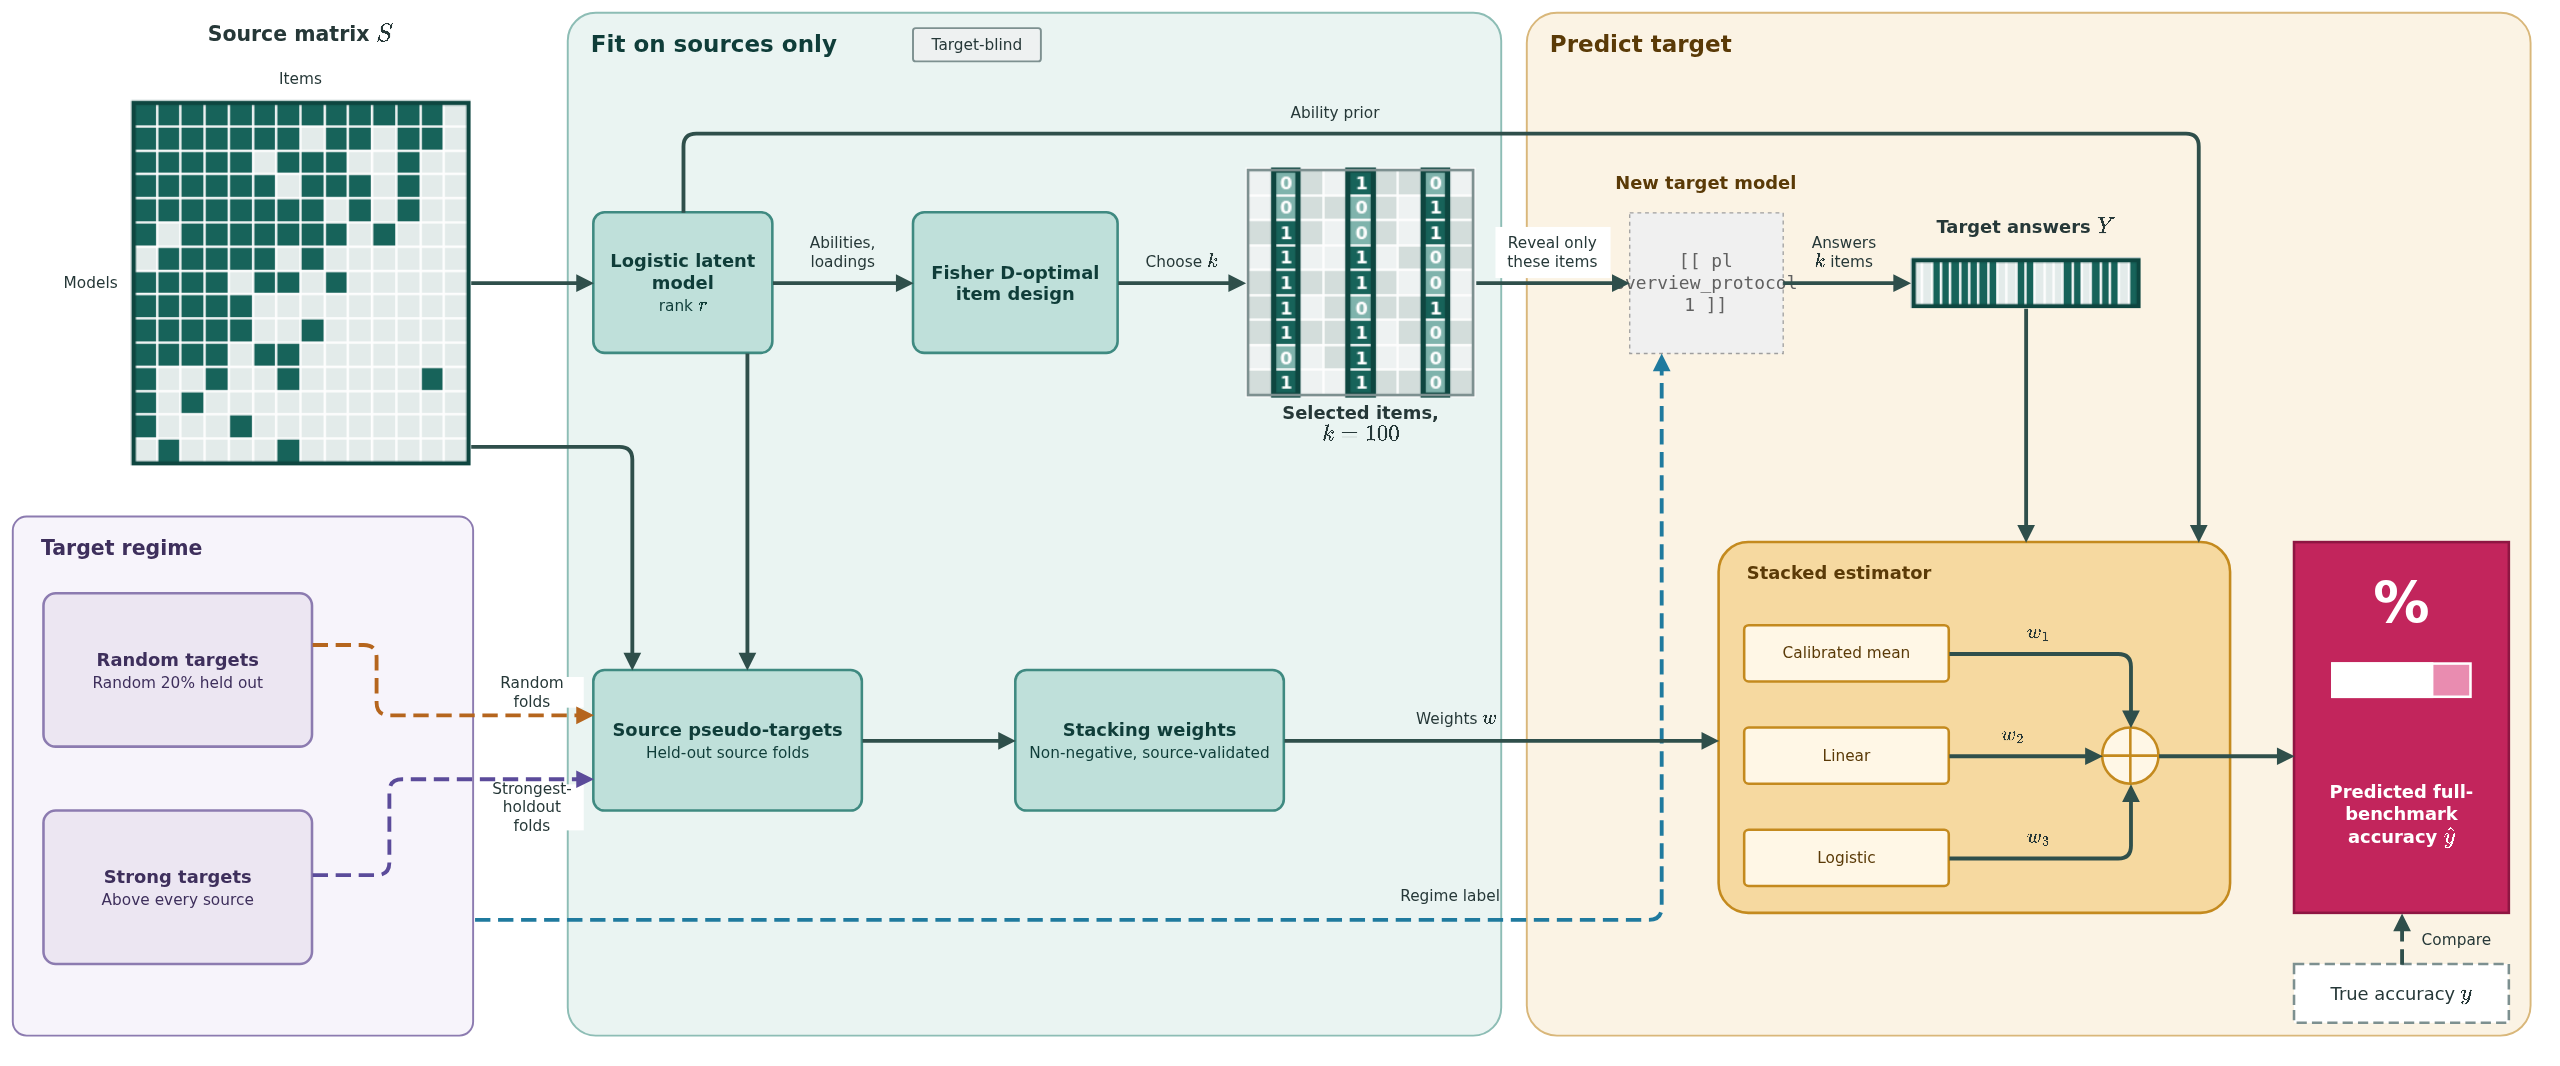
\includegraphics[width=\textwidth]{figures/overview_protocol.png}
\caption{Overview of the few-item prediction protocol and the evaluated configuration. A binary source matrix is used to fit a latent model, choose $k{=}100$ items, and fit stacking weights on source pseudo-targets; a new model answers only the selected items, and a stacked estimator predicts its full-benchmark accuracy. Targets are either random held-out models or models stronger than every source.}
\label{fig:overview}
\end{figure}

\section{Related Work}
\paragraph{Subset selection for benchmark prediction.} Anchor points \citep{Vivek2023AnchorPB} cluster items by the response vectors of source models and score a new model by a cluster-size-weighted average over representative items. tinyBenchmarks \citep{Polo2024tinyBenchmarksEL} combines such anchors with item response theory (IRT) to predict full scores, and metabench \citep{Kipnis2024metabenchA} uses IRT-based information to select items and fits a predictor on top of them. Efficient benchmarking \citep{Perlitz2023EfficientB} studies how much a large benchmark can be reduced while preserving model rankings, and PromptEval \citep{Polo2024EfficientME} applies related methods to the variation introduced by prompt formats. ONEBench \citep{Ghosh2024ONEBenchTT} studies how to aggregate sparse sample-level measurements into model scores and rankings. Our baselines follow the clustering and IRT families; the baseline implementations are the evaluator's own re-implementations rather than the original code.

\paragraph{Learned and adaptive prediction.} Pacchiardi et al.\ \citep{Pacchiardi2024100II} train an assessor that predicts a new model's success on unseen instances from its results on a few reference instances. Active evaluation acquisition \citep{Li2024ActiveEA} learns a policy that chooses items adaptively and predicts the rest. Adaptive testing in the psychometric tradition \citep{Zhuang2023PositionAE} and its extension to continuous scores \citep{Balkir2026ConfidentRW} choose items sequentially with stopping rules. Our setting is static: the $k$ items are chosen before seeing the target, from source data alone. A comparison of several benchmark-prediction methods across many benchmarks is reported by Zhang et al.\ \citep{Zhang2025HowBP}, whose released per-item score matrices we use as data (Section~\ref{sec:protocol}); we make no claim about their methods or conclusions beyond what the matrices contain.

\paragraph{Estimation and design tools.} The latent model is an IRT-style logistic model \citep{Rodriguez2021EvaluationEA} fitted to a model-by-item matrix; with a vector of abilities per model and item-specific loadings it is a compensatory multidimensional IRT model, whose item information and ability estimation are treated in \citet{Reckase2009MultidimensionalIR}, and the item-information criterion we use for selection is the same quantity that drives item selection in adaptive testing \citep{Zhuang2023PositionAE}. The final estimator follows the model-assisted approach of survey sampling, which corrects a model-based prediction with the mean residual of an observed sample, and which has been extended to flexible machine-learned predictors \citep{Breidt2017ModelAssistedSE}; prediction-powered inference \citep{Angelopoulos2023PredictionpoweredI} is a recent descendant of the same principle. Item selection by greedy log-determinant maximization is D-optimal experimental design \citep{Kiefer1960TheEO}, and the combination of estimators with non-negative weights fitted on held-out predictions is stacked generalization \citep{Wolpert1992StackedG}. Benchmark scores themselves vary with seeds and prompts \citep{Madaan2024QuantifyingVI}, which motivates reporting uncertainty for the gain over simple baselines.

\paragraph{Benchmarks.} The data comprise per-item outcomes on HELM-derived and Open LLM Leaderboard-derived benchmarks \citep{Liang2022HolisticEO}: development benchmarks IFEval \citep{Zhou2023InstructionFollowingEF}, ARC-Challenge \citep{Clark2018ThinkYH}, MuSR \citep{Sprague2023MuSRTT}, GSM8K \citep{Cobbe2021TrainingVT} and BBH \citep{Suzgun2022ChallengingBT}; and held-out benchmarks GPQA \citep{Rein2023GPQAAG}, MedQA \citep{Jin2020WhatDD}, LegalBench \citep{Guha2023LegalBenchAC}, MMLU \citep{Hendrycks2020MeasuringMM} and MMLU-Pro \citep{Wang2024MMLUProAM}.

\section{Setting and Method}
\label{sec:method}
\subsection{Problem setup}
For a benchmark with $n$ items, let $S\in\{0,1\}^{m\times n}$ be the binary correctness matrix of $m$ source models. A \emph{target} model is a new model whose per-item results are hidden except on a chosen subset. The procedure has two steps. A \emph{selector} sees only $S$ (with opaque item indices) and returns $k{=}100$ distinct item indices. The evaluator then reveals the targets' answers $Y\in\{0,1\}^{t\times k}$ on those items only, and a \emph{predictor} returns a predicted full-benchmark accuracy $\hat y_j$ for each target $j$. The reference is the target's true full accuracy $y_j$. Per episode we compute MAE, RMSE, Spearman and Kendall correlation between $\hat y$ and $y$ across the targets of that episode. Targets are drawn in one of two regimes: \emph{random targets} (a random 20\% of models, sources are the rest) and \emph{strong targets} (targets drawn from models whose full accuracy is at or above the 0.7 quantile; sources are the models strictly below it, so every target exceeds every source). The regime label is supplied to the candidate estimator with the source data; the baseline functions in the evaluator take only the source matrix and the target responses on their chosen items (\texttt{source\_evidence/evaluate\_final.py}, baseline functions).

\subsection{Design rationale}
The configuration is motivated by three observations; we state them as motivation, not as demonstrated mechanisms, because no single-factor ablation was run (Section~\ref{sec:discussion}).
(i) Binary outcomes saturate: a linear latent model can predict probabilities outside $[0,1]$ and must be clipped, whereas a logistic model keeps item probabilities calibrated and naturally describes how an item discriminates between abilities.
(ii) Under a logistic model an item's contribution to the information about a target's ability is $p(1-p)\,a a^{\top}$, which is largest near $p=0.5$. Evaluating this at reference abilities in the \emph{upper tail} of the source abilities, rather than at the centre, favours items that remain informative for strong targets.
(iii) Every hyperparameter and the estimator weights must be chosen without target information. Pseudo-targets inside the source set provide this: random folds mimic in-range targets, while holding out the strongest source models mimics out-of-range targets.

\subsection{Selected estimator}
Implementation details below are taken from the readable source of the evaluated configuration (\texttt{source\_evidence/candidate\_program.py}; the extension of Table~\ref{tab:search} is in \texttt{source\_evidence/extension\_program.py}).
\paragraph{Latent model.} A rank-$r$ logistic model, $\operatorname{logit}P_{mi}=b_i+a_i^{\top}\theta_m$, is fitted to $S$ by alternating L2-regularized Newton sweeps over item parameters $(b_i,a_i)$ and source abilities $\theta_m$, initialized from the SVD of the centred matrix. The empirical mean and covariance of the source abilities define a Gaussian prior for target abilities. A linear SVD-based latent model (item means, loadings, per-item residual variance, ridge/MAP ability) is fitted as well and serves as a stack member.

\paragraph{Item design.} Candidate designs of exactly $k$ items are generated: difficulty-stratified selection, a greedy Bayesian D-optimal design over linear-model item loadings, hybrids with a $k$-means medoid half, and three Fisher designs under the logistic model (pure, half stratified, half linear D-optimal). The Fisher design greedily maximizes $\log\det$ of $\tau\,\Sigma_\theta^{-1}+\sum_{i\in\text{design}} \bar w_i a_i a_i^{\top}$, with $\bar w_i$ the mean of $p_i(1-p_i)$ over reference abilities taken from the top 10\% of source abilities along the direction of increasing accuracy, shifted by $\{0,0.5,1\}$ standard deviations beyond it.

\paragraph{Target estimate.} For a target with answers $Y$ on items $\mathcal I$, ability is the MAP estimate under the Gaussian prior (Newton iterations on the $k$ answers). The model-assisted estimate, with and without a residual correction, is
\[
\hat y_{\text{plain}} = \frac1n\Big(\sum_{i\in\mathcal I} Y_i+\sum_{i\notin\mathcal I}\hat p_i\Big),\qquad
\hat y_{\text{corr}} = \hat y_{\text{plain}} + \frac{n-k}{n}\,\overline{(Y-\hat p)_{\mathcal I}},
\]
where $\hat p_i$ is the model probability and the correction adds the mean residual of the revealed items, extrapolated to the unrevealed items. A third estimator is the \emph{calibrated mean}: a linear map, fitted on source models, from subset mean to full accuracy.

\paragraph{Source-validated stacking.} For each design, rank, prior scale and residual-correction choice, predictions are made on source pseudo-targets: five random folds for random targets, or two folds that hold out the strongest 20\% and 10\% of sources for strong targets. Non-negative least squares with a heavily weighted sum-to-one row gives weights (summing to approximately one) over the calibrated mean, the linear estimate and the logistic estimate. Among the fifteen configurations with lowest pseudo-target error, the one minimizing a normalized RMSE plus rank-loss objective is retained. The calibrated mean on a stratified design is always in the search space, and any numerical failure or time-out of the logistic fit falls back to the simpler configuration. No target information enters selection or weights.

\subsection{Compared approaches}
\textbf{Baselines} (evaluator-owned re-implementations, same $k=100$, same episodes): \emph{random mean}, the target's mean over $k$ random items; \emph{anchor points}, $k$-means with $k$ clusters on item response columns of the source matrix, medoid anchors weighted by cluster size; and \emph{IRT-style}, a three-dimensional logistic IRT model fitted by Adam (200 iterations; \texttt{evaluate\_final.py}, \texttt{IRT\_DIMS}, \texttt{IRT\_ITERS}), $k$-means on item parameters to pick anchors, a ridge-regularized maximum-likelihood ability, and the mean predicted probability over all items. A fourth reference predicts the constant source mean and is used only inside the negative controls.

\textbf{Within-family variants} (development benchmarks only): a linear model-assisted D-optimal estimator without the logistic model or Fisher design (the stack's fallback member), the selected stacked configuration, and an extension that adds bagged posterior-mean probabilities and a tail-calibration column to the stack. These differ by cumulative changes, not single factors, and are reported as such.

\section{Experimental Protocol}
\label{sec:protocol}
\paragraph{Data.} Binary per-item outcome matrices (models $\times$ items) come from the public per-item score release accompanying \citet{Zhang2025HowBP}, built from the Open LLM Leaderboard and HELM. Five benchmarks were available for development (IFEval, ARC-Challenge, MuSR, GSM8K, BBH) and five disjoint benchmarks were reserved for the sealed final evaluation (GPQA, MedQA, LegalBench, MMLU, MMLU-Pro). The development evaluation uses seeds 11 and 12 (22 episodes including two controls); the final evaluation uses seeds 9101--9103 (32 episodes including two controls). Item order is randomly permuted per benchmark and seed. The target count is the larger of 5 and 20\% of the models; every episode requires at least 40 sources.

\paragraph{Utility score and aggregation.} Per episode, utility is $u=0.5\,\mathrm{clip}(1-2\,\mathrm{MAE},0,1)+0.5\,(\rho+1)/2$ with $\rho$ the Spearman correlation across targets. Episodes are averaged over seeds within each (benchmark, regime), then over benchmarks with equal weight, then over regimes with weights $0.5/0.5$. MAE, RMSE, Spearman and Kendall in the tables use the same hierarchy. Gains over baselines use the sign convention that positive favours the candidate: $\Delta\mathrm{MAE}=\mathrm{MAE}_{\text{baseline}}-\mathrm{MAE}_{\text{cand}}$ and $\Delta u=u_{\text{cand}}-u_{\text{baseline}}$. The best baseline is the one with the highest utility; this is the random-subset mean, so gains against ``the best baseline'' and against the random mean coincide.

\paragraph{Uncertainty.} For the gain over the best baseline we report a paired hierarchical bootstrap (300 replicates; resampling benchmarks, then seeds within benchmark, then target models within episode; 95\% percentile interval; bootstrap seed 20260101; \texttt{source\_evidence/evaluate\_final.py}, \texttt{bootstrap\_deltas}). Only five benchmarks and three seeds are resampled, so the interval is coarse. No interval is available for the anchor-point and IRT-style gains, and baseline-specific Spearman values are not part of the retained outputs; we do not infer significance for those comparisons.

\paragraph{Controls and qualification.} Two negative controls replace the target responses on the selected items: a permutation that assigns each target another target's answers, and a constant response pattern equal to the source majority. The final evaluation is labeled \emph{qualified} by the evaluator, with completed status and 32 of 32 episodes completed. We read this label as a statement about the evaluation outcome only, not as evidence of superiority or generalization. The evidence files mark the candidate-side diagnostics as unverified and provide no gate-level diagnostics, so we do not state which criteria underlie the label and attribute nothing to any individual criterion.

\section{Results}
\label{sec:results}
\subsection{Held-out comparison with baselines}
Table~\ref{tab:final} and Figure~\ref{fig:main} report the sealed evaluation on the five held-out benchmarks. All 32 episodes completed and none failed. The stacked configuration reaches MAE 0.0294, RMSE 0.0354, Spearman 0.843 and Kendall 0.715 (utility 0.9314). % @evidence[[derived/metrics_summary.json#final.mae]]
Baseline MAEs, derived as candidate MAE plus the reported gain, are 0.0339 (random mean), 0.0428 (anchor points) and 0.0692 (IRT-style); the corresponding point-estimate gains are $+0.0045$, $+0.0134$ and $+0.0398$. % @evidence[[derived/metrics_summary.json#final.baseline_mae_derived]]
The utility gain over the best baseline is $+0.0093$. The point estimates therefore favour the candidate over all three baselines.

The interval, however, does not resolve the comparison that matters most. The 95\% bootstrap interval for the MAE gain over the random-subset mean is $[-0.0052,+0.0134]$ and for the utility gain $[-0.0143,+0.0354]$; both contain zero. % @evidence[[derived/metrics_summary.json#final.ci_lo_delta_mae_vs_best_baseline]]
We therefore describe the gain as a modest point-estimate improvement that is not statistically resolved with five benchmarks and three seeds. The larger gains over anchor points and the IRT-style estimator cannot be assessed for significance with the retained outputs. The IRT-style baseline is a fixed-configuration re-implementation (three latent dimensions, 200 optimizer iterations); its weak result should not be read as a verdict on IRT-based prediction in general.

\begin{figure}[t]
\centering
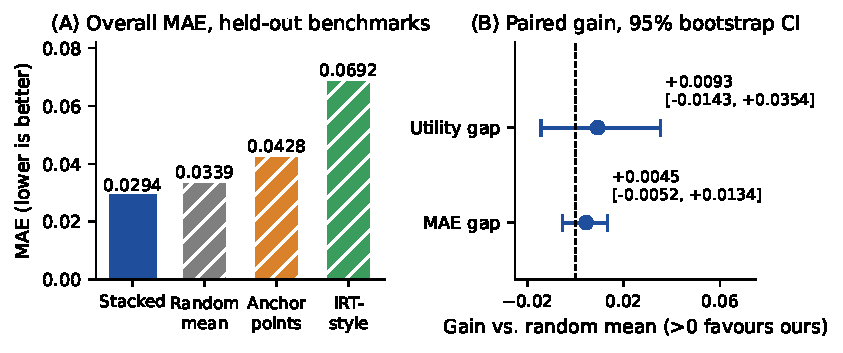
\includegraphics[width=\textwidth]{figures/main_comparison.pdf}
\caption{Held-out final evaluation (five benchmarks, three seeds, $k{=}100$). (A) Overall MAE of the stacked configuration and three baselines; baseline bars (hatched) are derived as candidate MAE plus the evaluator-reported gain. (B) Paired gain over the best baseline (the random-subset mean) in MAE and utility, with 95\% hierarchical bootstrap intervals; both intervals include zero.}
\label{fig:main}
\end{figure}

\begin{table}[t]
\centering
\caption{Sealed final evaluation on held-out benchmarks (five benchmarks, seeds 9101--9103, $k{=}100$). Gains are positive when the stacked configuration is better. ``Derived'' baseline MAEs equal candidate MAE plus the reported gain.}
\label{tab:final}
\small
\begin{tabular}{lcc}
\toprule
Quantity & Value & 95\% CI \\
\midrule
MAE / RMSE & 0.0294 / 0.0354 & --- \\ % @evidence[[derived/metrics_summary.json#final.rmse]]
Spearman / Kendall & 0.843 / 0.715 & --- \\
Utility & 0.9314 & --- \\
Utility per seed (9101 / 9102 / 9103) & 0.9257 / 0.9324 / 0.9360 & --- \\ % @evidence[[derived/metrics_summary.json#final.per_seed_utility]]
MAE, random / strong targets & 0.0179 / 0.0409 & --- \\
Spearman, random / strong targets & 0.956 / 0.730 & --- \\
\midrule
MAE gain vs.\ random mean (best baseline) & $+0.0045$ & $[-0.0052,+0.0134]$ \\
Utility gain vs.\ best baseline & $+0.0093$ & $[-0.0143,+0.0354]$ \\
MAE gain vs.\ anchor points & $+0.0134$ & not available \\
MAE gain vs.\ IRT-style & $+0.0398$ & not available \\
\midrule
Permuted: Spearman drop / MAE rise & 1.157 / 0.156 & --- \\ % @evidence[[derived/metrics_summary.json#final.control_permuted_mae_increase]]
Constant: MAE rise & 0.094 & --- \\
Episodes completed / failed & 32 / 0 & --- \\
\bottomrule
\end{tabular}
\end{table}

\subsection{Extrapolation to targets stronger than all sources}
Figure~\ref{fig:gap} separates the two regimes. On the held-out benchmarks, MAE is 0.0179 for random targets and 0.0409 for strong targets, a factor of about 2.3, and Spearman correlation falls from 0.956 to 0.730. % @evidence[[derived/metrics_summary.json#final.spearman_strong_targets]]
On the development benchmarks, the selected configuration shows the same pattern: MAE 0.0185 versus 0.0359 and Spearman 0.963 versus 0.816. % @evidence[[derived/metrics_summary.json#search.c02.mae_strong_targets]]
The gap is therefore not an artefact of one benchmark group, although it is larger on the held-out group. Even with a design aimed at upper-tail abilities and pseudo-target folds that hold out the strongest sources, strong-target ranking is much worse than random-target ranking; the configuration does not solve extrapolation. Because per-regime baseline results are not part of the retained outputs, we cannot say whether the gain over baselines is concentrated in one regime, nor whether baselines suffer a similar gap. Part of the regime difference may reflect statistical structure rather than extrapolation as such: strong targets occupy a narrower range of true scores, which by itself lowers rank correlation for a given prediction error. We did not test this.

\begin{figure}[t]
\centering
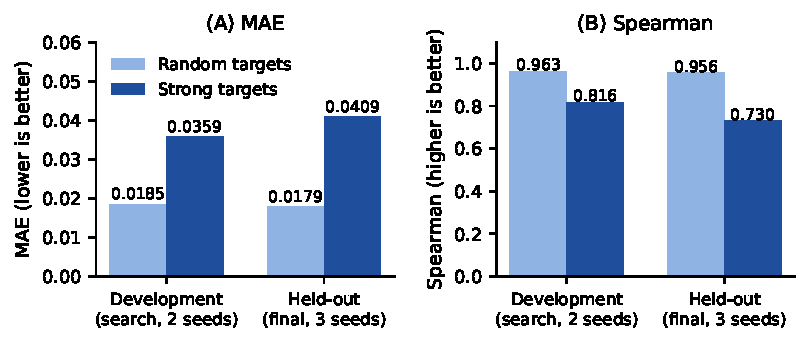
\includegraphics[width=\textwidth]{figures/extrapolation_gap.pdf}
\caption{Error and rank correlation by target regime for the selected stacked configuration. Development benchmarks (search evaluation, two seeds) and held-out benchmarks (final evaluation, three seeds) are different benchmark sets and are never pooled. (A) MAE. (B) Spearman correlation across targets.}
\label{fig:gap}
\end{figure}

\subsection{Negative controls}
Permuting target answers across targets raises MAE by 0.156 and lowers Spearman by 1.157 relative to the matched real episode, and replacing answers by a constant pattern raises MAE by 0.094. % @evidence[[derived/metrics_summary.json#final.control_constant_mae_delta]]
Predictions therefore depend on the target's revealed answers, as one would require of a valid estimator. The controls do not measure accuracy. Each control is a single episode matched to one real random-target episode, on one benchmark (MMLU-Pro) and the first seed of the final evaluation (\texttt{source\_evidence/evaluate\_final.py}, episode plan), so the control deltas carry no benchmark or seed variance.

\subsection{Within-family variants on development benchmarks}
Table~\ref{tab:search} compares the three configurations of the family on the development benchmarks (two seeds each; all three were scored, none failed). The utility is 0.9381 for the linear model-assisted estimator, 0.9452 for the selected stack and 0.9445 for the stack with bagged posterior means and tail calibration. % @evidence[[derived/metrics_summary.json#search.c02.combined_score]]
The difference between the latter two (0.0006) is smaller than the seed-to-seed spread inside a variant (for the selected stack, 0.9423 versus 0.9480), so the choice of the selected stack over its extension is a frozen choice, not a demonstrated superiority. The extension, which targets strong-target error, did not improve it (strong-target MAE 0.0362 versus 0.0359; Spearman 0.812 versus 0.816), which is consistent with the interpretation that additional tail correction fitted on source pseudo-targets adds nothing measurable here. The gain from the linear estimator to the stack (+0.0071 utility) is larger than the spread but arises from three simultaneous changes (logistic model, Fisher design, stacking) and two seeds, so it cannot be attributed to any component.

\begin{table}[t]
\centering
\caption{Development benchmarks (five benchmarks, seeds 11 and 12, $k{=}100$): three configurations of the same estimator family. The first row is the linear model-assisted estimator; the second is the configuration carried to the held-out evaluation; the third adds bagged posterior means and tail calibration. Utility is the aggregate defined in Section~\ref{sec:protocol}. Full metrics are in Table~\ref{tab:search-full}.}
\label{tab:search}
\small
\begin{tabular}{lcccc}
\toprule
Configuration & Utility & Per-seed utility (11 / 12) & MAE rand / strong & Spearman strong \\
\midrule
Linear model-assisted & 0.9381 & 0.9369 / 0.9393 & 0.0180 / 0.0389 & 0.771 \\
Stack (selected) & 0.9452 & 0.9423 / 0.9480 & 0.0185 / 0.0359 & 0.816 \\
Stack + tail calibration & 0.9445 & 0.9423 / 0.9468 & 0.0185 / 0.0362 & 0.812 \\
\bottomrule
\end{tabular}
\end{table}

\subsection{Search versus held-out performance}
The selected configuration's utility is 0.9452 on the development benchmarks and 0.9314 on the held-out benchmarks. The benchmark sets, seeds, and number of seeds differ, so we report the difference without a causal explanation. The MAE gain over the random mean is also larger on development benchmarks ($+0.0086$) than on held-out benchmarks ($+0.0045$). % @evidence[[derived/metrics_summary.json#search.c02.delta_mae_vs_random_mean]]
Development scores are proxies that influenced which configuration was frozen; held-out scores are the appropriate basis for any claim.

\section{Discussion and Limitations}
\label{sec:discussion}
\paragraph{What the evidence supports.} The stacked configuration has lower point-estimate MAE than three matched baselines on five held-out benchmarks, predictions that degrade as expected under both negative controls (each a single episode; no pass/fail criterion for the controls is evidenced), and shows a large degradation for stronger-than-source targets. It does not establish a statistically resolved improvement over a random-subset mean, a superiority claim, or generalization to other benchmarks, budgets or score types. The evaluator's ``qualified'' label is not a superiority or generalization claim, and no gate-level diagnostics are available to interpret it further.

\paragraph{Attribution.} The configuration differs from the random-mean baseline in four ways at once: items are selected using source data, a source-fitted calibration maps subset means to full accuracy, latent-model predictions are blended in, and the regime label selects the validation folds. No experiment isolates these. The gain over random mean could come from calibration alone, from item selection, or from the latent models; the benefit of the Fisher design under upper-tail reference abilities, in particular, is untested. The regime label is not given to the baselines, so the candidate has information they lack; this should be kept in mind when reading the comparison.

\paragraph{Threats to validity.} (i) Five benchmarks and three seeds make the bootstrap coarse; a larger panel might show a clear gain or none. (ii) Targets within an episode are few for some benchmarks, so Spearman and Kendall are noisy per episode. (iii) The strong-target regime is one definition (above the 0.7 accuracy quantile, sources below it) and need not represent real future models. (iv) Baselines are the evaluator's re-implementations with fixed settings; stronger tuned versions might narrow the gap. (v) Selection of the configuration used development scores from two seeds with within-variant spread comparable to between-variant differences. (vi) Candidate diagnostics are marked unverified.

\paragraph{Practical reading.} For a user who only needs coarse model scores on benchmarks resembling the historical pool, the random-target numbers (MAE 0.0179, Spearman 0.956 at $k=100$) indicate that 100 items can recover full accuracy to within about two percentage points on average and keep rankings largely intact. % @evidence[[derived/metrics_summary.json#final.mae_random_targets]]
For a user who must rank systems that exceed everything in the historical pool, the strong-target numbers (MAE 0.0409, Spearman 0.730) indicate that subset predictions alone should be treated as screening information, with direct evaluation reserved for the decisions that matter. Whether the stacked configuration or a plain random-subset mean is preferable for this purpose cannot be decided from our evidence, because their difference is smaller than the uncertainty we measured; the random mean is simpler, needs no source data, and has no regime-dependent tuning.

\paragraph{Relation to published numbers.} We do not compare against numbers reported in earlier papers: protocols differ in benchmark sets, target definitions, item budgets and metrics, and our baselines are re-implementations with fixed settings rather than the original code. Conclusions here are limited to the matched comparison on the evaluator's episodes.

\paragraph{What would resolve the comparison.} The width of the MAE-gain interval (0.0186) is about four times its point estimate (0.0045), so the held-out panel is too small to distinguish a gain of this size from zero. A decisive test would need more benchmarks and seeds than the five and three used here, paired in the same way, together with per-regime baseline results so that any gain can be located in the in-range or out-of-range regime. We expect, but have not verified, that the sign of the gain is more stable than its magnitude.

\paragraph{Not tested.} A sweep over the item budget $k$, additional seeds, single-factor ablations (latent rank, prior shrinkage, logistic versus linear model, Fisher versus stratified design, stacking versus a single estimator), temporal or model-family splits, and non-binary scores were not run. These are the experiments needed to attribute any gain to a mechanism.

\section{Conclusion}
We evaluated a source-validated stacked latent-ability estimator with Fisher D-optimal item design for predicting a new model's full-benchmark accuracy from 100 items. On five held-out benchmarks it had the lowest point-estimate MAE among the compared estimators (0.0294 versus 0.0339 for the random-subset mean) and its predictions degraded as expected under both negative controls (single episodes; no pass/fail criterion is evidenced), but the interval for its gain over the best baseline spans zero, so the improvement is not statistically established. The largest measured difference is that targets stronger than every source model are predicted about twice as badly (MAE 0.0409, Spearman 0.730) as random targets (MAE 0.0179, Spearman 0.956), on both development and held-out benchmark groups (point estimates, without intervals, and possibly partly due to the narrower score range of strong targets), and the design aimed at upper-tail abilities did not close this gap. Practically, a user who needs to rank models stronger than the historical pool should not rely on source-matrix-based subset prediction without direct validation on a few full evaluations. Future work should test a budget sweep, single-factor ablations and per-regime baseline comparisons to learn which component, if any, helps, and whether item selection can be made robust for out-of-range targets.

% IMPORTANT: \clearpage flushes all pending floats before references so that
% body-page counting excludes reference-only pages.  Do NOT remove.
\clearpage
\bibliography{references}
\bibliographystyle{paper}

\clearpage
\appendix
\section{Supplementary Information}

\subsection{Evaluation protocol and metric definitions}
Each episode is identified by a seed, a benchmark and a regime. For random targets the evaluator draws as targets 20\% of the $M$ models with results on the benchmark (rounded to the nearest integer, at least 5) and uses the rest as sources. For strong targets, the pool is the set of models with full accuracy at or above the 0.7 quantile; sources are models strictly below it, and the targets are drawn from the pool (at most the same number). Episodes require at least 40 sources and 5 targets. The source matrix is transferred in at most two chunks of bit-packed rows (\texttt{source\_evidence/evaluate\_final.py}, \texttt{MAX\_LOAD\_CHUNKS}, \texttt{pack\_bits}). The selector must return exactly $k{=}100$ distinct valid indices, and the predictor must return one finite prediction per target. Aggregation proceeds from seeds to benchmarks (equal weight) to regimes (0.5/0.5); failed or missing episodes would contribute worst-case values, but none occurred in either evaluation (22 and 32 episodes completed, 0 failed). The development benchmarks are IFEval, ARC-Challenge, MuSR, GSM8K and BBH; the held-out benchmarks are GPQA, MedQA, LegalBench, MMLU and MMLU-Pro. The number of observed candidate calls was 88 in the development evaluation and 128 in the final evaluation.

\subsection{Estimator details of the selected configuration}
\begin{itemize}
\item \textbf{Linear latent model:} centred source matrix, SVD of the $m\times m$ Gram matrix, maximum rank 12; item residual variances are floored at $\max(0.02,\text{5th percentile})$. Rank grid $\{1,2,3,5,8,12\}$ and prior-scale grid $\tau\in\{1,4,16\}$.
\item \textbf{Logistic latent model:} eight alternating Newton sweeps with L2 penalties 0.5 (loadings), 0.05 (intercepts) and 1.0 (abilities); steps clipped to $[-2,2]$; rank grid $\{2,3,1,5\}$ evaluated in that order under a 45-second budget for logistic fitting, after which remaining ranks are skipped; prior-scale grid $\{1,4,16\}$; target abilities by up to 15 Newton iterations.
\item \textbf{Designs:} four linear designs (stratified; stratified$+$D-optimal half; D-optimal; $k$-means$+$D-optimal half) and three Fisher designs (pure; half stratified; half linear D-optimal), the latter built at logistic rank 3 with reference abilities from the top 10\% of source abilities plus margins $\{0,0.5,1.0\}$ standard deviations.
\item \textbf{Blend grid:} linear or logistic estimator blended with the calibrated mean with weights $\{0,0.2,\dots,1\}$, plus NNLS stacks over the three best linear and three best logistic candidates per design.
\item \textbf{Selection objective:} among the 15 lowest-MSE pseudo-target configurations, minimize $\mathrm{RMSE}/\mathrm{RMSE}_{\min}+(1-\overline{(\rho+\tau)/2})$, with the rank term averaged over folds.
\item \textbf{Fallbacks:} if validation cannot run (fewer than ten source models) a conservative blend of 0.7 calibrated mean and 0.3 linear estimate on a hybrid design is used; any exception returns a stratified design with the calibrated mean.
\end{itemize}
The values above are constants and routines in \texttt{source\_evidence/candidate\_program.py} (constant block and the functions \texttt{fit\_logistic\_latent}, \texttt{\_make\_folds}, \texttt{\_validate}, \texttt{stack\_weights}). The extension in Table~\ref{tab:search} (\texttt{source\_evidence/extension\_program.py}) additionally uses bagged logistic fits at ranks 2, 3 and 4, a Laplace posterior mean for item probabilities, and a ridge-shrunk monotone tail correction applied only above the source median accuracy, accepted only if it beats the incumbent on pseudo-targets.

\subsection{Development-benchmark results for all three configurations}
\begin{table}[h]
\centering
\caption{Complete development-benchmark metrics (five benchmarks, seeds 11 and 12). Gains are positive when the configuration is better than the baseline. Rows: linear model-assisted estimator; selected stack; stack with tail calibration.}
\label{tab:search-full}
\footnotesize
\setlength{\tabcolsep}{3pt}
\begin{tabular}{lccc}
\toprule
Metric & Linear & Stack (selected) & Stack + tail \\
\midrule
Utility & 0.9381 & 0.9452 & 0.9445 \\ % @evidence[[derived/metrics_summary.json#search.c01.combined_score]]
MAE / RMSE & 0.0285 / 0.0347 & 0.0272 / 0.0336 & 0.0274 / 0.0339 \\
Spearman / Kendall & 0.866 / 0.730 & 0.889 / 0.756 & 0.888 / 0.752 \\
MAE random / strong & 0.0180 / 0.0389 & 0.0185 / 0.0359 & 0.0185 / 0.0362 \\
Spearman random / strong & 0.962 / 0.771 & 0.963 / 0.816 & 0.963 / 0.812 \\
MAE gain vs.\ random mean & $+0.0073$ & $+0.0086$ & $+0.0084$ \\
MAE gain vs.\ anchor points & $+0.0096$ & $+0.0109$ & $+0.0107$ \\
MAE gain vs.\ IRT-style & $+0.0405$ & $+0.0418$ & $+0.0416$ \\
Utility gain vs.\ best baseline & $+0.0084$ & $+0.0155$ & $+0.0148$ \\
Permuted: Spearman drop / MAE increase & 1.021 / 0.109 & 1.033 / 0.110 & 1.033 / 0.110 \\
Constant: MAE increase & 0.077 & 0.077 & 0.077 \\
\bottomrule
\end{tabular}
\end{table}

\subsection{Final evaluation details}
The per-seed utilities of the selected configuration are 0.9257 (seed 9101), 0.9324 (seed 9102) and 0.9360 (seed 9103); their spread (0.0103) is comparable to the point-estimate utility gain over the best baseline (0.0093), consistent with the unresolved bootstrap interval. % @evidence[[derived/metrics_summary.json#final.per_seed_utility]]
Recorded wall-clock time per seeded run was 150.8, 77.4 and 75.1 seconds respectively for the three seeds. The evaluator reports 128 candidate calls observed over 32 episodes. Utility differences against anchor points and IRT-style baselines are not accompanied by intervals in the retained outputs. The evaluation was declared \emph{qualified} with completed status; candidate-side diagnostics are recorded as unverified.

\subsection{Reproducibility, data provenance and seeds}
\textbf{Data.} The per-item matrices are the public score files released with \citet{Zhang2025HowBP}, pinned to a fixed repository commit (55faff49\ldots{}), derived from the Open LLM Leaderboard and HELM. \textbf{Seeds.} Development 11, 12; final 9101, 9102, 9103; bootstrap 20260101; the evaluated configuration seeds its own generators from the episode seed. \textbf{Software.} The task requirements file (\texttt{source\_evidence/requirements.txt}) pins numpy 2.5.4, scipy 1.18.1, scikit-learn 1.9.1 and joblib 1.6.0; the evaluated configuration sets eight BLAS threads by default (\texttt{candidate\_program.py}, header). \textbf{Figures.} Figures~\ref{fig:main} and \ref{fig:gap} are produced by a single plotting script from the evaluator outputs and the retained metrics files; the overview figure is a schematic and contains no data. \textbf{Code.} The numbers derive from a single-file estimator and the evaluator script, whose baselines are the evaluator's own implementations; copies of the sources are supplied under \texttt{source\_evidence/} and are not linked in this anonymized draft. We did not access the raw leaderboard details, which are partly gated.

\subsection{LLM Usage}
Large language models were used throughout this work. An LLM-based research agent proposed the estimator variants, implemented them, ran the development and final evaluations through the provided harness, selected related work from a starter list and retrieved references, and drafted this manuscript. All reported numbers originate from the evaluator outputs and retained metric files, not from model generation; the LLM did not generate data. The agent did not access any content excluded by the task rules.

\end{document}
